\setcounter{secnumdepth}{5}

\chapter{Ambiente di lavoro}

\section{Docker: container}

Docker è una tecnologia di conteinerizzazione open source che permette la creazione e l'utilizzo dei container Linux®. La tecnologia Docker utilizza il kernel di Linux e le sue funzionalità. 

\subsection{Perchè docker?}
La scelta è ricaduta in docker poiché permette di creare numerosi container con un'esigua quantità di memoria necessaria per l'esecuzione.

\subsection{Dockerfile}
Un Dockerfile è un documento di testo che contiene tutti i comandi che un utente può chiamare sulla riga di comando per assemblare un'immagine. 

Esempio di Dockerfile:
\begin{figure}[h]
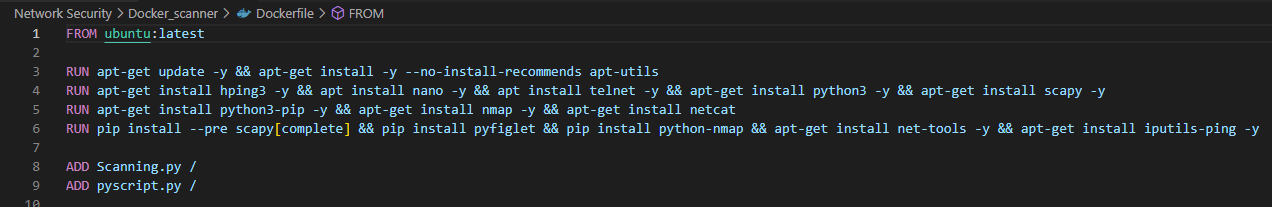
\includegraphics[scale=0.4]{UNINA_MSc_Thesis_Project/img/Dockerfile scanner.png}
\caption{Esempio dockerfile: Scanner}
\end{figure}

\section{Docker Security Playground}
Docker security playground è un framework grafico che permette la creazione e la gestione di reti contenenti container docker. 

\begin{figure}[h]
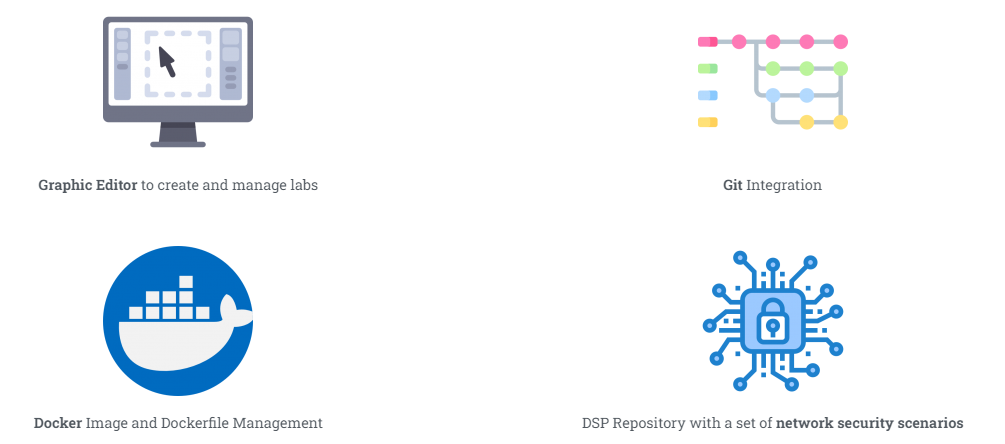
\includegraphics[scale=0.3]{UNINA_MSc_Thesis_Project/img/DSP_Features.png}
\centering
\caption{Features DSP}
\end{figure}

Per l'utilizzo, esso necessita di: \textit{Nodejs, git, docker, docker-compose e strumenti di compilazione c++/g++} e si presenta come in figura: 
\begin{figure}[h]
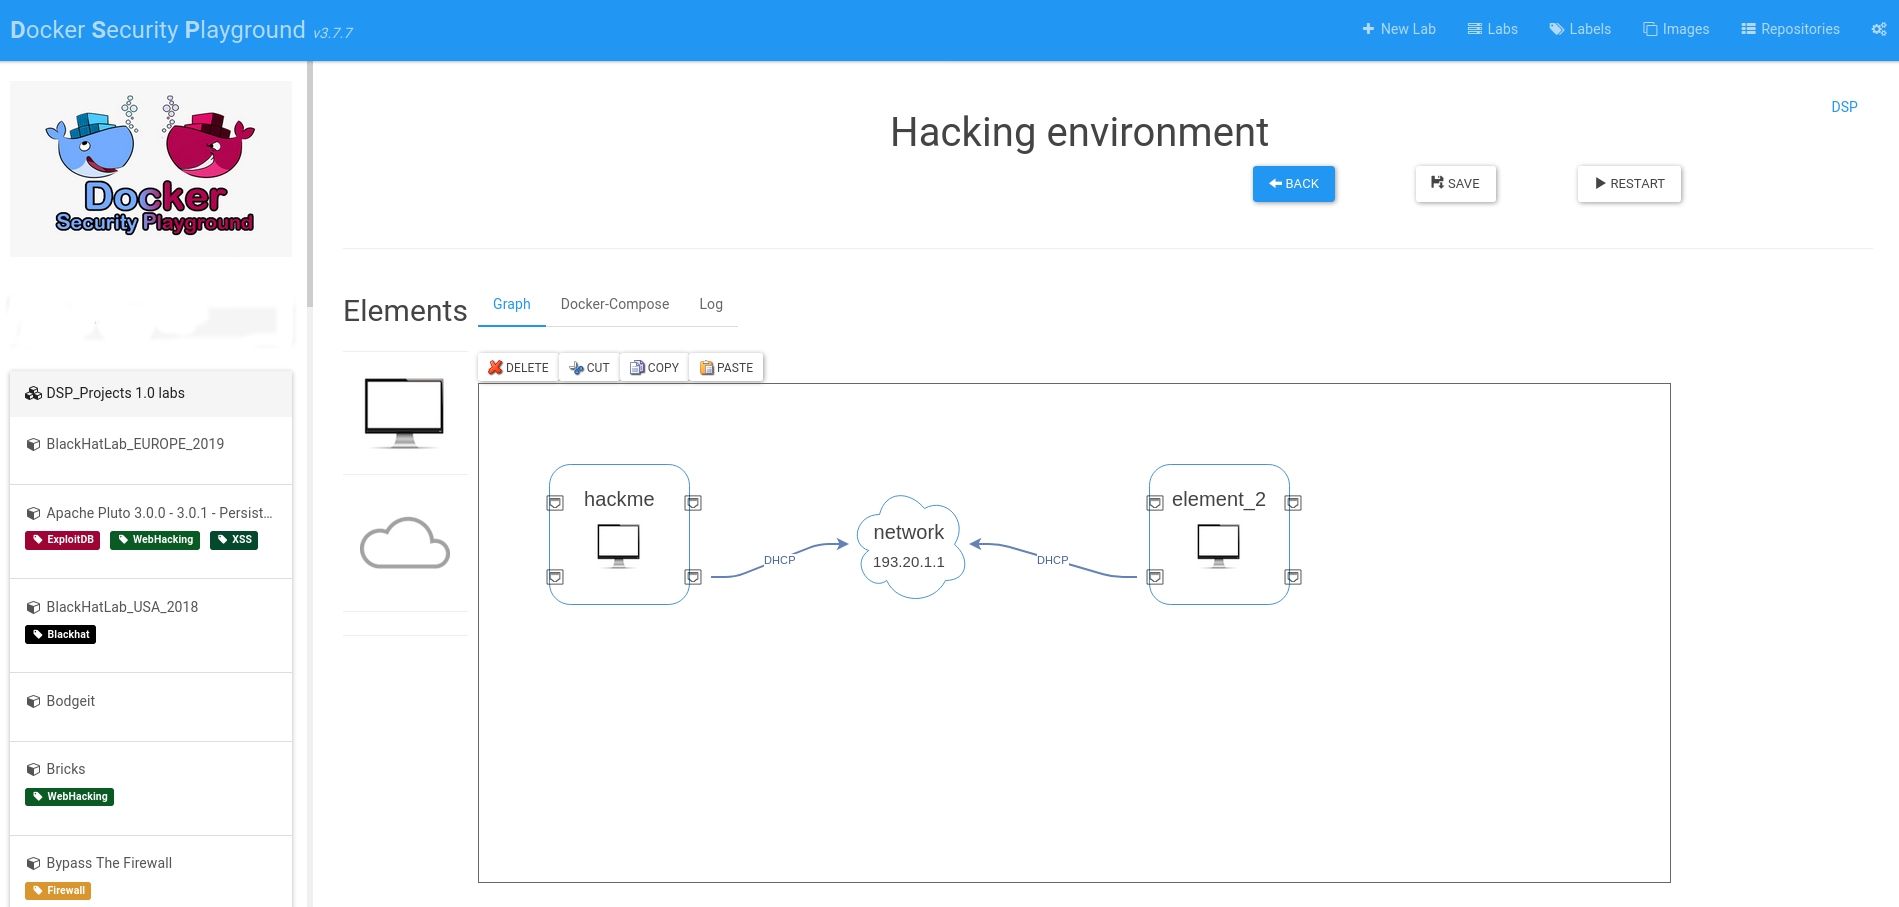
\includegraphics[scale=0.18]{UNINA_MSc_Thesis_Project/img/DSP_comesipresenta.png}
\centering
\caption{DSP: come si presenta}
\end{figure}

\section{Python: scapy}
Scapy è un potente \textit{programma interattivo di manipolazione dei pacchetti}. È in grado di falsificare o decodificare pacchetti di un ampio numero di protocolli, inviarli, catturarli, abbinare richieste e risposte e molto altro ancora. E' possibile utilizzare scapy su python attraverso il download e l'utilizzo della libreria ufficiale \textbf{scapy}.

Il comando più importante di scapy, in questo contesto, è il comando sr (send-receive), descritto in figura:
\begin{figure}[h]
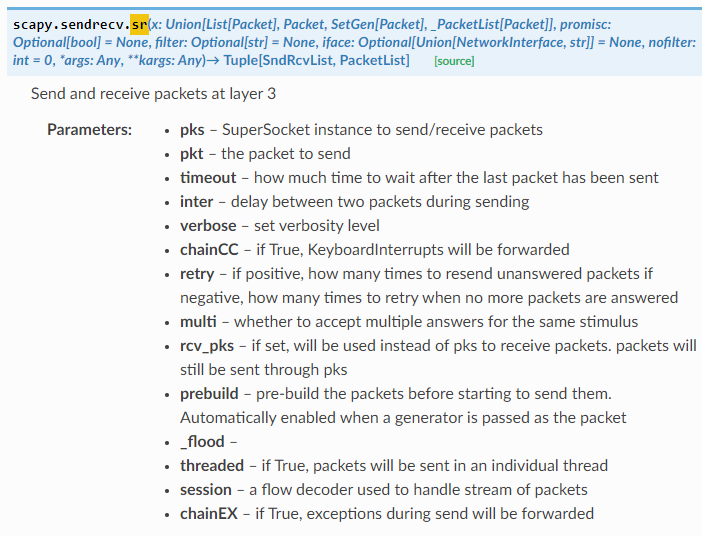
\includegraphics[scale=0.60]{UNINA_MSc_Thesis_Project/img/scapy_sr.png}
\centering
\caption{scapy "sr()"}
\end{figure}

